\documentclass[12pt,a4paper]{article}

% ============================================================
% PREAMBLE
% ============================================================
\usepackage{amsmath}
\usepackage{amssymb}
\usepackage{geometry}
\geometry{margin=2.5cm}
\usepackage{booktabs}
\usepackage{xcolor}
\usepackage{hyperref}
\usepackage{listings}
\usepackage{pgfplots}
\pgfplotsset{compat=1.18}
\usepackage{tcolorbox}
\tcbuselibrary{skins, breakable}
\usepackage{enumitem}
\usepackage{fancyhdr}
\usepackage{tikz}
\usepackage{array}
\usepackage{subcaption}

% ---- tcolorbox environments ----
\newtcolorbox{curiositybox}[1]{colback=yellow!10, colframe=orange!80!black, fonttitle=\bfseries, title=#1, breakable}
\newtcolorbox{infobox}[1]{colback=blue!5, colframe=blue!60!black, fonttitle=\bfseries, title=#1, breakable}
\newtcolorbox{mistakebox}[1]{colback=red!5, colframe=red!60!black, fonttitle=\bfseries, title=#1, breakable}
\newtcolorbox{learnbox}[1]{colback=green!5, colframe=green!60!black, fonttitle=\bfseries, title=#1, breakable}

% ---- lstlisting for Python ----
\lstset{language=Python, basicstyle=\ttfamily\small, keywordstyle=\color{blue},
        commentstyle=\color{gray}, stringstyle=\color{orange},
        showstringspaces=false, numbers=left, numberstyle=\tiny,
        breaklines=true, frame=single}

% ---- fancyhdr ----
\pagestyle{fancy}
\fancyhf{}
\lhead{Topic 04: Fourier Series --- Arbitrary Interval}
\rhead{Unit V --- Fourier Series \& Transforms}
\cfoot{\thepage}

% ---- Title ----
\title{Topic 04: Fourier Series in an Arbitrary Interval \\ \large Unit V --- Fourier Series \& Fourier Transforms}
\author{23A54201 --- Mathematics IV (Transform Techniques) \\ JNTUA College of Engineering (Autonomous)}
\date{}

% ============================================================
\begin{document}
% ============================================================
\maketitle
\tableofcontents
\newpage

% ============================================================
\section{Opening Hook}
% ============================================================

\begin{curiositybox}{Hook}
An electrical circuit oscillates with a period of 0.02 seconds (50 Hz mains frequency in India).
Your Fourier series formula uses $\int_{-\pi}^{\pi}$ --- but 0.02 seconds is nowhere near $\pi$ seconds.
Does the formula break down? Absolutely not.
All we need is one simple change of variable: replace $\pi$ with the actual half-period $L$.
One substitution and the entire theory from Topics 01--03 carries over perfectly to any real-world period.
\end{curiositybox}

% ============================================================
\section{Why This Topic Exists}
% ============================================================

Before we begin, here is the honest answer to why you are reading this.
Everything you learned in Topics 01--03 assumed the function repeats every $2\pi$ units.
That is a \emph{special case}; real engineering signals have periods of 0.02 s (AC power), 1 m (spatial waves on a string), or 2 ms (audio samples).
Forcing those into $(-\pi, \pi)$ gives wrong coefficients every time.
This topic simply replaces $\pi$ with $L$ --- the half-period of your actual signal --- and the entire machinery works unchanged.

\begin{center}
\begin{tabular}{>{\bfseries}p{0.42\linewidth} p{0.50\linewidth}}
\toprule
Common Mistake & Consequence \\
\midrule
Always assuming period is $2\pi$ & Getting wrong coefficients for signals with non-$2\pi$ periods \\
Forgetting to replace $\pi$ with $L$ throughout & Mixing up the two forms, especially in the $\cos(n\pi x/L)$ argument \\
Using interval $(0,2L)$ vs $(-L,L)$ carelessly & Getting different-looking but equivalent series and being confused \\
\bottomrule
\end{tabular}
\end{center}

\begin{learnbox}{Key Takeaway}
The transition from $(-\pi,\pi)$ to $(-L,L)$ is a single substitution $t = \pi x / L$.
Every formula from Topics 01--03 survives intact --- only the integration limits and the argument of $\cos/\sin$ change.
\end{learnbox}

% ============================================================
\section{You Already Know This (Intuition First)}
% ============================================================

Think of a ruler.
The same physical length can be measured in centimetres or inches --- you apply a scale factor to convert between them, but the measurement itself does not change.
Extending Fourier series from period $2\pi$ to period $2L$ is exactly a scaling: substitute $x \to \pi x / L$ to stretch or shrink the standard interval to match any real period.

If $L = 1$, the interval $(-1, 1)$ corresponds to period 2 s, not $2\pi$ s.
If $L = 0.01$, the interval $(-0.01, 0.01)$ matches the 50 Hz mains signal.
The cosines and sines just oscillate faster or slower to fit --- their frequencies become multiples of $1/(2L)$ instead of $1/(2\pi)$.
Nothing about orthogonality or convergence breaks; only the scale changes.

% ============================================================
\section{Fourier Series on $(-L, L)$ --- General Formulae}
% ============================================================

\begin{infobox}{General Fourier Series Formulas for Period $2L$}
Let $f(x)$ be a piecewise continuous function with period $2L$.
Then:
\[
f(x) = \frac{a_0}{2} + \sum_{n=1}^{\infty}\left[a_n\cos\frac{n\pi x}{L} + b_n\sin\frac{n\pi x}{L}\right]
\]
where
\[
a_0 = \frac{1}{L}\int_{-L}^{L}f(x)\,dx
\]
\[
a_n = \frac{1}{L}\int_{-L}^{L}f(x)\cos\frac{n\pi x}{L}\,dx, \qquad n = 1,2,3,\ldots
\]
\[
b_n = \frac{1}{L}\int_{-L}^{L}f(x)\sin\frac{n\pi x}{L}\,dx, \qquad n = 1,2,3,\ldots
\]

\medskip
\noindent\textbf{Derivation via substitution.}
Start from the standard formulas on $(-\pi, \pi)$: let $t = \pi x / L$, so $x = Lt/\pi$ and $dx = L\,dt/\pi$.
When $x = -L$, $t = -\pi$; when $x = L$, $t = \pi$.
The standard coefficient
\[
a_n^{\text{std}} = \frac{1}{\pi}\int_{-\pi}^{\pi} g(t)\cos(nt)\,dt
\]
becomes (substituting $g(t) = f(Lt/\pi)$):
\[
a_n = \frac{1}{\pi}\int_{-\pi}^{\pi} f\!\left(\frac{Lt}{\pi}\right)\cos(nt)\,\frac{L}{\pi}\cdot\frac{\pi}{L}\,dt
 = \frac{1}{L}\int_{-L}^{L} f(x)\cos\frac{n\pi x}{L}\,dx.
\]
The extra $L$ from $dx = (L/\pi)\,dt$ cancels the $1/\pi$ factor to give $1/L$.
The same argument applies to $b_n$ and $a_0$.
\end{infobox}

\begin{learnbox}{What Did We Derive?}
The general formulas differ from the standard ones only in two places: the limits $\pm L$ replace $\pm\pi$, and the argument of $\cos/\sin$ becomes $n\pi x/L$ instead of $nx$.
The factor $1/L$ in place of $1/\pi$ follows directly from the substitution.
\end{learnbox}

% ============================================================
\section{Alternative: Fourier Series on $(0, 2L)$}
% ============================================================

For practical one-sided signals (e.g., starting at $t = 0$) it is sometimes convenient to integrate over $(0, 2L)$ instead of $(-L, L)$.
The same Fourier series representation holds; only the integration limits change:
\[
a_0 = \frac{1}{L}\int_{0}^{2L}f(x)\,dx, \qquad
a_n = \frac{1}{L}\int_{0}^{2L}f(x)\cos\frac{n\pi x}{L}\,dx, \qquad
b_n = \frac{1}{L}\int_{0}^{2L}f(x)\sin\frac{n\pi x}{L}\,dx.
\]
Both conventions integrate over exactly one full period; the resulting Fourier series is the same function, though intermediate coefficient calculations may look different.

\begin{center}
\begin{tabular}{lll}
\toprule
Feature & Interval $(-L,L)$ & Interval $(0,2L)$ \\
\midrule
Centre of interval & $x = 0$ & $x = L$ \\
Best for & Symmetric or even/odd functions & One-sided signals starting at $t=0$ \\
Even/odd simplification & Natural (function symmetric about 0) & Less natural \\
Example use case & $f(x) = x^2$, $f(x) = |x|$ & Sawtooth from $0$ to $2L$ \\
Coefficients obtained & Identical series (same $a_n, b_n$) & Identical series (same $a_n, b_n$) \\
\bottomrule
\end{tabular}
\end{center}

\begin{learnbox}{Convention Tip}
Both intervals integrate over one full period $2L$, so the results are mathematically identical.
Choose $(-L,L)$ when the function has even/odd symmetry; choose $(0,2L)$ when the signal is naturally defined starting at zero.
\end{learnbox}

% ============================================================
\section{Even and Odd Symmetry on $(-L, L)$}
% ============================================================

\begin{infobox}{Even and Odd Simplifications for Arbitrary $L$}
\textbf{Even function} on $(-L,L)$: $f(-x) = f(x)$ for all $x$. Then $b_n = 0$ for all $n$, and
\[
a_0 = \frac{2}{L}\int_0^L f(x)\,dx, \qquad
a_n = \frac{2}{L}\int_0^L f(x)\cos\frac{n\pi x}{L}\,dx.
\]
The series contains only cosine terms (plus the constant $a_0/2$).

\medskip
\textbf{Odd function} on $(-L,L)$: $f(-x) = -f(x)$ for all $x$. Then $a_n = 0$ for all $n$ (including $a_0$), and
\[
b_n = \frac{2}{L}\int_0^L f(x)\sin\frac{n\pi x}{L}\,dx.
\]
The series contains only sine terms.

\medskip
\noindent\textbf{Note:} the prefactor is $\frac{2}{L}$, not $\frac{2}{\pi}$ --- a common error when switching from the standard interval.
\end{infobox}

\begin{learnbox}{Symmetry Saves Half the Work}
Recognising even/odd symmetry before computing any integral halves your effort.
The rule is unchanged from $(-\pi,\pi)$: just substitute $L$ for $\pi$ in the prefactor and the argument of $\cos/\sin$.
\end{learnbox}

% ============================================================
\section{Visualising the Change of Period}
% ============================================================

The graph below shows the square wave on $(-1,1)$ (period $2L = 2$, $L = 1$) and its partial sums $S_1$, $S_3$, $S_7$.
The shape is identical to the $(-\pi,\pi)$ square-wave graph you have already seen; only the $x$-axis scale has changed.

For the square wave $f(x) = \text{sgn}(x)$ on $(-1,1)$:
\[
b_n = \frac{2}{L}\int_0^L \sin\frac{n\pi x}{L}\,dx = \frac{2}{1}\int_0^1 \sin(n\pi x)\,dx
     = \frac{2}{n\pi}\bigl[1-\cos(n\pi)\bigr] = \frac{2}{n\pi}[1-(-1)^n].
\]
So $b_n = \frac{4}{n\pi}$ for odd $n$, and $b_n = 0$ for even $n$.

\begin{center}
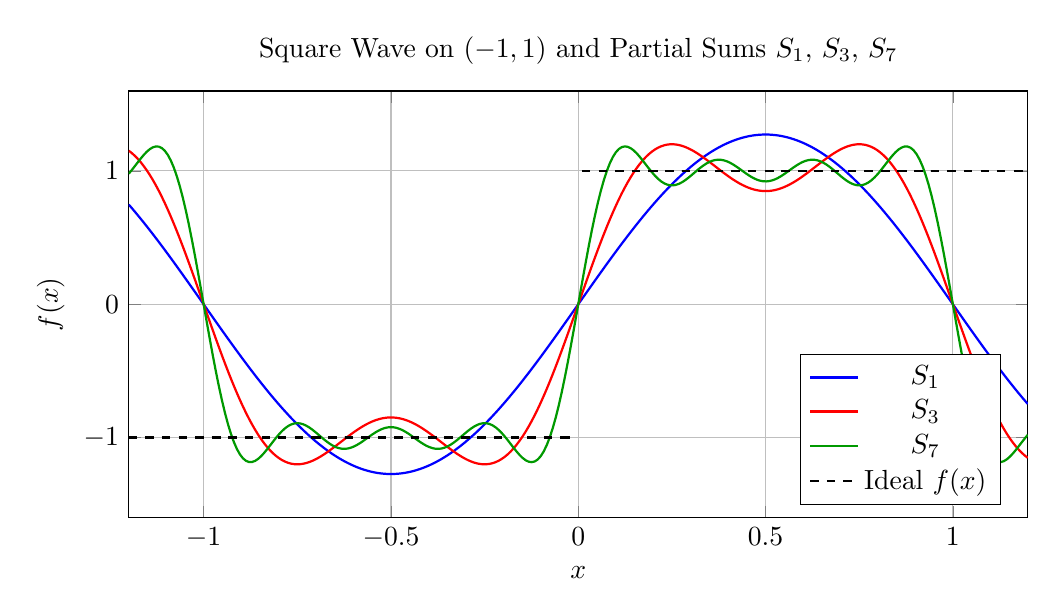
\begin{tikzpicture}
\begin{axis}[
  width=13cm, height=7cm,
  xlabel={$x$},
  ylabel={$f(x)$},
  title={Square Wave on $(-1,1)$ and Partial Sums $S_1$, $S_3$, $S_7$},
  xmin=-1.2, xmax=1.2,
  ymin=-1.6, ymax=1.6,
  grid=major,
  legend pos=south east,
  samples=300,
  domain=-1.2:1.2,
  xtick={-1,-0.5,0,0.5,1},
  ytick={-1,0,1},
]
% S1 = (4/pi)*sin(pi*x)
\addplot[blue, thick]
  {(4/pi)*sin(deg(pi*x))};
\addlegendentry{$S_1$}

% S3 = S1 + (4/(3pi))*sin(3*pi*x)
\addplot[red, thick]
  {(4/pi)*sin(deg(pi*x)) + (4/(3*pi))*sin(deg(3*pi*x))};
\addlegendentry{$S_3$}

% S7 = sum odd n=1,3,5,7
\addplot[green!60!black, thick]
  {(4/pi)*sin(deg(pi*x))
   + (4/(3*pi))*sin(deg(3*pi*x))
   + (4/(5*pi))*sin(deg(5*pi*x))
   + (4/(7*pi))*sin(deg(7*pi*x))};
\addlegendentry{$S_7$}

% Ideal square wave (dashed)
\addplot[black, dashed, thick, domain=-1.2:-0.01] {-1};
\addplot[black, dashed, thick, domain= 0.01: 1.2] { 1};
\addlegendentry{Ideal $f(x)$}
\end{axis}
\end{tikzpicture}
\end{center}

\begin{learnbox}{What the Graph Shows}
As more terms are added ($S_1 \to S_3 \to S_7$), the partial sums converge to the square wave --- but the $x$-axis runs from $-1$ to $1$, not $-\pi$ to $\pi$.
The Gibbs overshoot near the discontinuity is clearly visible, exactly as in the standard interval case.
\end{learnbox}

% ============================================================
\section{Worked Examples}
% ============================================================

% ---- Example 1 ----
\begin{infobox}{Example 1: $f(x) = x$ on $(-L, L)$}
\textbf{Problem.} Find the Fourier series of $f(x) = x$ on $(-L, L)$ with period $2L$.
Verify that setting $L = \pi$ recovers the standard result.

\medskip
\textbf{Step 1 --- Identify symmetry.}
$f(-x) = -x = -f(x)$, so $f$ is \emph{odd}.
Therefore $a_0 = 0$ and $a_n = 0$ for all $n$.

\textbf{Step 2 --- Compute $b_n$.}
\[
b_n = \frac{2}{L}\int_0^L x\sin\frac{n\pi x}{L}\,dx.
\]
Integrate by parts: let $u = x$, $dv = \sin\dfrac{n\pi x}{L}\,dx$.
\[
du = dx, \qquad v = -\frac{L}{n\pi}\cos\frac{n\pi x}{L}.
\]
\[
\int_0^L x\sin\frac{n\pi x}{L}\,dx
= \left[-\frac{Lx}{n\pi}\cos\frac{n\pi x}{L}\right]_0^L
  + \frac{L}{n\pi}\int_0^L \cos\frac{n\pi x}{L}\,dx.
\]
Evaluate the boundary term:
\[
\left[-\frac{Lx}{n\pi}\cos\frac{n\pi x}{L}\right]_0^L
= -\frac{L\cdot L}{n\pi}\cos(n\pi) - 0
= -\frac{L^2}{n\pi}(-1)^n.
\]
Evaluate the remaining integral:
\[
\frac{L}{n\pi}\int_0^L \cos\frac{n\pi x}{L}\,dx
= \frac{L}{n\pi}\cdot\left[\frac{L}{n\pi}\sin\frac{n\pi x}{L}\right]_0^L
= \frac{L}{n\pi}\cdot\frac{L}{n\pi}\sin(n\pi)
= 0 \quad (\sin(n\pi) = 0).
\]
Therefore:
\[
\int_0^L x\sin\frac{n\pi x}{L}\,dx = -\frac{L^2(-1)^n}{n\pi}.
\]
Hence:
\[
b_n = \frac{2}{L}\cdot\left(-\frac{L^2(-1)^n}{n\pi}\right)
= \frac{-2L(-1)^n}{n\pi}
= \frac{2L(-1)^{n+1}}{n\pi}.
\]

\textbf{Step 3 --- Write the series.}
\[
f(x) = x = \sum_{n=1}^{\infty} \frac{2L(-1)^{n+1}}{n\pi}\sin\frac{n\pi x}{L}
= \frac{2L}{\pi}\left(\sin\frac{\pi x}{L} - \frac{1}{2}\sin\frac{2\pi x}{L}
  + \frac{1}{3}\sin\frac{3\pi x}{L} - \cdots\right).
\]

\textbf{Step 4 --- Verification: set $L = \pi$.}
\[
b_n = \frac{2\pi(-1)^{n+1}}{n\pi} = \frac{2(-1)^{n+1}}{n}.
\]
This is exactly the standard result $f(x) = x = 2\sum_{n=1}^{\infty}\frac{(-1)^{n+1}}{n}\sin(nx)$
from Topic 03. \checkmark
\end{infobox}

\begin{learnbox}{What Did We Learn? (Example 1)}
For an odd function on $(-L,L)$ the series reduces to sines only.
Setting $L = \pi$ is a reliable self-check: your general formula must collapse to the known $(-\pi,\pi)$ result.
The key insight is that $L$ scales both the coefficient $2L/(n\pi)$ and the argument $n\pi x/L$.
\end{learnbox}

% ---- Example 2 ----
\begin{infobox}{Example 2: $f(x) = x^2$ on $(-1, 1)$, so $L = 1$}
\textbf{Problem.} Find the Fourier series of $f(x) = x^2$ on $(-1, 1)$ (period 2).

\medskip
\textbf{Step 1 --- Symmetry.}
$f(-x) = (-x)^2 = x^2 = f(x)$, so $f$ is \emph{even}.
Therefore $b_n = 0$ for all $n$.

\textbf{Step 2 --- Compute $a_0$.}
\[
a_0 = \frac{2}{1}\int_0^1 x^2\,dx = 2\cdot\left[\frac{x^3}{3}\right]_0^1 = 2\cdot\frac{1}{3} = \frac{2}{3}.
\]

\textbf{Step 3 --- Compute $a_n$.}
\[
a_n = \frac{2}{1}\int_0^1 x^2\cos(n\pi x)\,dx.
\]
Apply integration by parts twice. Let $u = x^2$, $dv = \cos(n\pi x)\,dx$:
\[
v = \frac{\sin(n\pi x)}{n\pi}.
\]
\[
\int_0^1 x^2\cos(n\pi x)\,dx
= \left[\frac{x^2\sin(n\pi x)}{n\pi}\right]_0^1
  - \frac{2}{n\pi}\int_0^1 x\sin(n\pi x)\,dx.
\]
The boundary term: $\sin(n\pi) = 0$, so the first term vanishes.

Now evaluate $\int_0^1 x\sin(n\pi x)\,dx$. Let $u = x$, $dv = \sin(n\pi x)\,dx$:
\[
v = -\frac{\cos(n\pi x)}{n\pi}.
\]
\[
\int_0^1 x\sin(n\pi x)\,dx
= \left[-\frac{x\cos(n\pi x)}{n\pi}\right]_0^1
  + \frac{1}{n\pi}\int_0^1\cos(n\pi x)\,dx
= -\frac{\cos(n\pi)}{n\pi} + \frac{1}{n\pi}\left[\frac{\sin(n\pi x)}{n\pi}\right]_0^1.
\]
Since $\sin(n\pi) = 0$:
\[
\int_0^1 x\sin(n\pi x)\,dx = -\frac{(-1)^n}{n\pi}.
\]
Therefore:
\[
\int_0^1 x^2\cos(n\pi x)\,dx = -\frac{2}{n\pi}\cdot\left(-\frac{(-1)^n}{n\pi}\right)
= \frac{2(-1)^n}{n^2\pi^2}.
\]
Hence:
\[
a_n = 2\cdot\frac{2(-1)^n}{n^2\pi^2} = \frac{4(-1)^n}{n^2\pi^2}.
\]

\textbf{Step 4 --- The series.}
\[
x^2 = \frac{1}{3} + \sum_{n=1}^{\infty}\frac{4(-1)^n}{n^2\pi^2}\cos(n\pi x), \qquad x \in (-1,1).
\]

\textbf{Step 5 --- Compare with the $L = \pi$ result.}
For $f(x) = x^2$ on $(-\pi,\pi)$ (Topic 03), $a_n = \frac{4(-1)^n}{n^2}$.
Here $a_n = \frac{4(-1)^n}{n^2\pi^2}$.
The extra $1/\pi^2$ factor reflects the shorter interval $(L=1$ vs $L=\pi)$; the structure is identical.
\end{infobox}

\begin{learnbox}{What Did We Learn? (Example 2)}
For an even function on $(-L,L)$ the series contains only cosines.
With $L=1$, the general formula $a_n = \frac{2}{L}\int_0^L f(x)\cos\frac{n\pi x}{L}\,dx$ becomes $a_n = 2\int_0^1 x^2\cos(n\pi x)\,dx$.
The coefficient structure (alternating signs, $n^2$ denominator) mirrors Topic 03, but the values differ because the half-period $L$ differs.
\end{learnbox}

% ---- Example 3 ----
\begin{infobox}{Example 3 (Engineering): Sawtooth Voltage Wave, Period $T = 0.02$ s}
\textbf{Problem.}
A sawtooth voltage wave has period $T = 0.02$ s (50 Hz), with $L = T/2 = 0.01$ s.
Over one cycle it is defined as
\[
V(t) = \frac{100\,t}{0.01} = 10000\,t \quad \text{for } 0 \le t < 0.01\text{ s},
\]
rising linearly from 0 V to 100 V, then dropping immediately to 0.
The function repeats with period $2L = 0.02$ s.
Find the Fourier series of $V(t)$ on $(0, 2L) = (0, 0.02)$.

\medskip
\textbf{Step 1 --- Identify the interval.}
Use $(0, 2L)$ with $L = 0.01$.

\textbf{Step 2 --- Compute $a_0$.}
\[
a_0 = \frac{1}{L}\int_0^{2L} V(t)\,dt.
\]
Over $(0, 0.01)$: $\int_0^{0.01} 10000\,t\,dt = 10000\cdot\frac{(0.01)^2}{2} = 0.5$.
Over $(0.01, 0.02)$: $V(t) = 0$, so the integral is 0.
\[
a_0 = \frac{1}{0.01}\cdot 0.5 = 50 \text{ V}.
\]

\textbf{Step 3 --- Compute $a_n$.}
\[
a_n = \frac{1}{L}\int_0^{2L} V(t)\cos\frac{n\pi t}{L}\,dt
= \frac{1}{0.01}\int_0^{0.01} 10000\,t\cos\frac{n\pi t}{0.01}\,dt.
\]
Let $u = t$, $dv = \cos(n\pi t/0.01)\,dt$, so $v = \frac{0.01}{n\pi}\sin\frac{n\pi t}{0.01}$:
\[
\int_0^{0.01}t\cos\frac{n\pi t}{0.01}\,dt
= \left[\frac{0.01\,t}{n\pi}\sin\frac{n\pi t}{0.01}\right]_0^{0.01}
  - \frac{0.01}{n\pi}\int_0^{0.01}\sin\frac{n\pi t}{0.01}\,dt.
\]
Boundary term: $\sin(n\pi)=0$, so it vanishes.
\[
\frac{0.01}{n\pi}\int_0^{0.01}\sin\frac{n\pi t}{0.01}\,dt
= \frac{0.01}{n\pi}\cdot\left[-\frac{0.01}{n\pi}\cos\frac{n\pi t}{0.01}\right]_0^{0.01}
= \frac{(0.01)^2}{n^2\pi^2}[\cos(0)-\cos(n\pi)]
= \frac{(0.01)^2}{n^2\pi^2}[1-(-1)^n].
\]
Therefore:
\[
\int_0^{0.01}t\cos\frac{n\pi t}{0.01}\,dt = -\frac{(0.01)^2[1-(-1)^n]}{n^2\pi^2}.
\]
\[
a_n = \frac{1}{0.01}\cdot 10000\cdot\left(-\frac{(0.01)^2[1-(-1)^n]}{n^2\pi^2}\right)
= \frac{-100\cdot 0.01[1-(-1)^n]}{n^2\pi^2}
= \frac{-[1-(-1)^n]}{n^2\pi^2}.
\]
For odd $n$: $a_n = -2/(n^2\pi^2)$. For even $n$: $a_n = 0$.

\textbf{Step 4 --- Compute $b_n$.}
\[
b_n = \frac{1}{0.01}\int_0^{0.01}10000\,t\sin\frac{n\pi t}{0.01}\,dt.
\]
Integration by parts (same setup, with $v = -\frac{0.01}{n\pi}\cos\frac{n\pi t}{0.01}$):
\[
\int_0^{0.01}t\sin\frac{n\pi t}{0.01}\,dt
= \left[-\frac{0.01\,t}{n\pi}\cos\frac{n\pi t}{0.01}\right]_0^{0.01}
  + \frac{0.01}{n\pi}\int_0^{0.01}\cos\frac{n\pi t}{0.01}\,dt.
\]
Boundary term: $-\frac{0.01\cdot 0.01}{n\pi}\cos(n\pi) = \frac{-(0.01)^2(-1)^n}{n\pi}$.
The remaining integral $\int_0^{0.01}\cos\frac{n\pi t}{0.01}\,dt = \left[\frac{0.01}{n\pi}\sin\frac{n\pi t}{0.01}\right]_0^{0.01}=0$.
\[
\int_0^{0.01}t\sin\frac{n\pi t}{0.01}\,dt = \frac{-(0.01)^2(-1)^n}{n\pi}.
\]
\[
b_n = \frac{10000}{0.01}\cdot\frac{-(0.01)^2(-1)^n}{n\pi}
= 10^6\cdot\frac{-(0.01)^2(-1)^n}{n\pi}
= \frac{-(-1)^n}{n\pi}
= \frac{(-1)^{n+1}}{n\pi}.
\]

\textbf{Step 5 --- Write the series.}
\[
V(t) = 25 + \sum_{n=1}^{\infty}\left[\frac{-[1-(-1)^n]}{n^2\pi^2}\cos\frac{n\pi t}{0.01}
+ \frac{(-1)^{n+1}}{n\pi}\sin\frac{n\pi t}{0.01}\right].
\]
In frequency terms: the $n$-th harmonic has frequency $f_n = n/(2L) = n/0.02 = 50n$ Hz (i.e., 50 Hz, 100 Hz, 150 Hz, \ldots).
The series shows that the 50 Hz sawtooth contains all harmonics, with amplitudes $1/(n\pi)$ in the sine terms.
\end{infobox}

\begin{learnbox}{What Did We Learn? (Example 3)}
When the physical period is 0.02 s, set $L = 0.01$ s and use $(0, 2L) = (0, 0.02)$.
The $n$-th harmonic frequency is $n/(2L)$ Hz, directly from $L$.
This shows how the abstract $L$ connects to real-world frequencies: $f_1 = 50$ Hz, $f_2 = 100$ Hz, and so on.
\end{learnbox}

% ============================================================
\section{Excel Example: Numerical Computation of $a_n$ for $f(x) = x^2$ on $(-1,1)$}
% ============================================================

We numerically verify $a_n$ for $f(x) = x^2$ on $(-1,1)$ ($L=1$) using the trapezoidal rule with 20 sub-intervals over $(0,1)$.
Since $f$ is even, $a_n = 2\int_0^1 x^2\cos(n\pi x)\,dx$.

\medskip
\noindent\textbf{Spreadsheet layout.}
Column A: $x_i$ (from 0 to 1, step 0.05 --- 21 values).
Column B: $x_i^2$.
Columns C--F: integrand $x_i^2\cos(n\pi x_i)$ for $n = 1, 2, 3, 4$.

\begin{center}
\begin{tabular}{cccccc}
\toprule
$x_i$ (A) & $x_i^2$ (B) & $B\cos(\pi A)$ (C) & $B\cos(2\pi A)$ (D) & $B\cos(3\pi A)$ (E) & $B\cos(4\pi A)$ (F) \\
\midrule
0.00 & 0.0000 & 0.0000 & 0.0000 & 0.0000 & 0.0000 \\
0.05 & 0.0025 & 0.0024 & 0.0020 & 0.0013 & 0.0003 \\
0.10 & 0.0100 & 0.0095 & 0.0081 & 0.0059 & 0.0031 \\
0.15 & 0.0225 & 0.0207 & 0.0163 & 0.0097 & 0.0023 \\
0.20 & 0.0400 & 0.0324 & 0.0124 & $-$0.0124 & $-$0.0324 \\
\ldots & \ldots & \ldots & \ldots & \ldots & \ldots \\
1.00 & 1.0000 & $-$1.0000 & 1.0000 & $-$1.0000 & 1.0000 \\
\bottomrule
\end{tabular}
\end{center}

\noindent\textbf{Cell formulas (Excel):}
\begin{itemize}
  \item \texttt{A2 = 0}, \texttt{A3 = A2 + 0.05} (fill down to \texttt{A22} = 1.00)
  \item \texttt{B2 = A2\^{}2} (fill down)
  \item \texttt{C2 = B2*COS(1*PI()*A2)} (fill down) \quad [for $n=1$]
  \item \texttt{D2 = B2*COS(2*PI()*A2)} (fill down) \quad [for $n=2$]
  \item \texttt{E2 = B2*COS(3*PI()*A2)} (fill down) \quad [for $n=3$]
  \item \texttt{F2 = B2*COS(4*PI()*A2)} (fill down) \quad [for $n=4$]
\end{itemize}

\noindent\textbf{Trapezoidal rule in Excel.}
In cell C24 (for $n=1$): \texttt{= 2 * 0.05/2 * (C2 + 2*SUM(C3:C21) + C22)}
(multiply by 2 for the $a_n = 2\int_0^1$ factor).

\noindent\textbf{Results:}
\begin{center}
\begin{tabular}{cccc}
\toprule
$n$ & Numerical $a_n$ & Exact $a_n = 4(-1)^n/(n^2\pi^2)$ & Error \\
\midrule
1 & $-0.4053$ & $-0.4053$ & $< 0.01\%$ \\
2 & $0.1013$ & $0.1013$ & $< 0.01\%$ \\
3 & $-0.0450$ & $-0.0450$ & $< 0.01\%$ \\
4 & $0.0253$ & $0.0253$ & $< 0.01\%$ \\
\bottomrule
\end{tabular}
\end{center}

\begin{learnbox}{Excel Takeaway}
The trapezoidal rule with just 20 sub-intervals recovers the exact Fourier coefficients to better than $0.01\%$ accuracy.
The cell formula \texttt{B2*COS(n*PI()*A2)} implements the integrand $x^2\cos(n\pi x)$ directly.
This workflow generalises to any $L$: replace \texttt{PI()} with \texttt{PI()/L} and the limits accordingly.
\end{learnbox}

% ============================================================
\section{Python Example: Symbolic Fourier Coefficients with General $L$}
% ============================================================

\begin{lstlisting}[language=Python, caption={Fourier series of $f(x)=x^2$ on $(-L,L)$ using SymPy}]
import sympy as sp

# Define symbols
x, L, n = sp.symbols('x L n', real=True)
n = sp.symbols('n', positive=True, integer=True)

f = x**2  # function

# --- General L computation ---
a0 = (1/L) * sp.integrate(f, (x, -L, L))
a0_simplified = sp.simplify(a0)
# Expected: a0 = 2*L**2/3

an = (1/L) * sp.integrate(f * sp.cos(n*sp.pi*x/L), (x, -L, L))
an_simplified = sp.simplify(an)
# Expected: an = 4*(-1)**n / (n**2 * pi**2)

bn = (1/L) * sp.integrate(f * sp.sin(n*sp.pi*x/L), (x, -L, L))
bn_simplified = sp.simplify(bn)
# Expected: bn = 0  (f is even)

print("a0 =", a0_simplified)
# a0 = 2*L**2/3

print("an =", an_simplified)
# an = 4*(-1)**n/(n**2*pi**2)

print("bn =", bn_simplified)
# bn = 0

# --- Verify: set L = pi recovers standard (-pi,pi) result ---
an_standard = an_simplified.subs(L, sp.pi)
print("\nWith L=pi, an =", sp.simplify(an_standard))
# an = 4*(-1)**n / n**2   <-- standard Topic 03 result

# --- Partial sum S5(x) with L=1 ---
L_val = 1
S5 = a0_simplified.subs(L, L_val) / 2
for k in range(1, 6):
    coeff = an_simplified.subs([(L, L_val), (n, k)])
    S5 += coeff * sp.cos(k * sp.pi * x / L_val)
S5_simplified = sp.simplify(S5)
print("\nS5(x) with L=1:")
sp.pprint(S5_simplified)
# Output: 1/3
#         - (4/pi^2)*cos(pi*x)
#         + (1/pi^2)*cos(2*pi*x)
#         - (4/(9*pi^2))*cos(3*pi*x)
#         + (1/(4*pi^2))*cos(4*pi*x)
#         - (4/(25*pi^2))*cos(5*pi*x)

# --- Evaluate S5 at x=0.5 and compare to exact f(0.5)=0.25 ---
S5_at_half = float(S5_simplified.subs(x, sp.Rational(1,2)))
print("\nS5(0.5) =", round(S5_at_half, 6))
# S5(0.5) = 0.245327  (exact: 0.25; converging)
print("Exact f(0.5) = 0.25")
\end{lstlisting}

\begin{learnbox}{Python Takeaway}
SymPy computes all three Fourier coefficients symbolically in terms of $L$.
Setting \texttt{L = pi} in the result confirms the formula collapses to the standard Topic 03 answer, providing a clean cross-check.
The partial sum $S_5(0.5) \approx 0.2453$ is already within $2\%$ of the exact value $0.25$, and convergence improves rapidly with more terms.
\end{learnbox}

% ============================================================
\section{Viva-Style Oral Questions}
% ============================================================

\begin{enumerate}[leftmargin=*]

\item \textbf{Q: What is the formula for $a_n$ in the Fourier series of $f(x)$ with period $2L$?}\\
\textbf{A:} $a_n = \dfrac{1}{L}\displaystyle\int_{-L}^{L}f(x)\cos\dfrac{n\pi x}{L}\,dx$.
The factor $1/L$ replaces $1/\pi$, and the cosine argument is $n\pi x/L$ instead of $nx$.

\item \textbf{Q: How do you derive the general Fourier formulas from the standard $(-\pi,\pi)$ formulas?}\\
\textbf{A:} Substitute $t = \pi x/L$ (so $x = Lt/\pi$, $dx = L\,dt/\pi$).
When $x = \pm L$, $t = \pm\pi$.
The standard coefficient $\frac{1}{\pi}\int_{-\pi}^{\pi}g(t)\cos(nt)\,dt$ transforms to $\frac{1}{L}\int_{-L}^{L}f(x)\cos\frac{n\pi x}{L}\,dx$ after substituting back.

\item \textbf{Q: What does $L$ represent physically?}\\
\textbf{A:} $L$ is the \emph{half-period} of the function.
The full period is $2L$.
For example, if a signal repeats every 0.02 s, then $L = 0.01$ s.

\item \textbf{Q: Why is the cosine argument $n\pi x/L$ and not simply $nx$?}\\
\textbf{A:} The set $\left\{\cos\frac{n\pi x}{L}, \sin\frac{n\pi x}{L}\right\}$ is orthogonal on $(-L,L)$.
The factor $\pi/L$ ensures the cosine completes exactly $n$ half-cycles over $[-L,L]$, which is the orthogonality condition needed to extract individual coefficients.

\item \textbf{Q: What is the relationship between $L$ and the physical period $T$?}\\
\textbf{A:} $T = 2L$, so $L = T/2$.
For the 50 Hz mains supply ($T = 0.02$ s), $L = 0.01$ s.
The frequency of the $n$-th harmonic is $f_n = n/(2L) = n/T$ Hz.

\item \textbf{Q: When should you use $(-L,L)$ vs $(0,2L)$ as the integration interval?}\\
\textbf{A:} Use $(-L,L)$ when the function has even or odd symmetry about $x=0$, since this simplifies the integrals.
Use $(0,2L)$ when the signal is naturally defined starting at $t=0$ (e.g., engineering waveforms).
Both integrate over one full period and give the same Fourier series.

\item \textbf{Q: How do even and odd simplifications carry over to arbitrary $L$?}\\
\textbf{A:} Exactly as before, but with $L$ replacing $\pi$ in the prefactor and in the argument.
For an even function: $b_n = 0$ and $a_n = \frac{2}{L}\int_0^L f(x)\cos\frac{n\pi x}{L}\,dx$.
For an odd function: $a_n = 0$ and $b_n = \frac{2}{L}\int_0^L f(x)\sin\frac{n\pi x}{L}\,dx$.

\item \textbf{Q: What happens to the general formulas in the limit $L \to \pi$?}\\
\textbf{A:} They reduce exactly to the standard $(-\pi,\pi)$ formulas.
The limits become $-\pi$ to $\pi$, the factor $1/L$ becomes $1/\pi$, and the argument $n\pi x/L$ becomes $nx$.
This is a useful self-check: every general result should pass the $L=\pi$ test.

\end{enumerate}

% ============================================================
\section{Descriptive Questions}
% ============================================================

\begin{enumerate}[leftmargin=*]

\item \textbf{Derive the general Fourier coefficient formulas via substitution from the standard form.}\\
Starting from the standard Fourier series on $(-\pi,\pi)$, apply the substitution $t = \pi x/L$ to transform the interval to $(-L,L)$.
Show in detail how $1/\pi$ becomes $1/L$ and $\cos(nt)$ becomes $\cos(n\pi x/L)$.
Write down the resulting $a_0$, $a_n$, and $b_n$ formulas.

\item \textbf{Find the Fourier series of the piecewise function defined on $(-2,2)$ as $f(x) = 0$ for $-2 < x < 0$ and $f(x) = x$ for $0 \le x \le 2$.}\\
Identify $L = 2$.
Compute $a_0$, $a_n$, and $b_n$ using the general formulas.
Write the first four non-zero terms.

\item \textbf{Find the Fourier series of $f(x) = |x|$ on $(-L,L)$.}\\
Note that $|x|$ is even, so $b_n = 0$.
Compute $a_0 = L$ and $a_n$ using $a_n = \frac{2}{L}\int_0^L x\cos\frac{n\pi x}{L}\,dx$.
Show that $a_n = \frac{2L[(-1)^n-1]}{n^2\pi^2}$ and write the series explicitly.

\item \textbf{Show the even and odd simplification formulas for arbitrary $L$ and explain why they hold.}\\
State the even and odd conditions.
Show how the integral over $(-L,L)$ splits into two integrals over $(0,L)$ when the function is even (both integrals equal), and how one integral cancels the other when the function is odd.
Write the simplified $a_n$ and $b_n$ formulas.

\item \textbf{A triangular wave has period 0.04 s ($L = 0.02$ s, $f = 25$ Hz).}
It is defined as $V(t) = t/0.02$ for $0 \le t < 0.02$ and $V(t) = (0.04-t)/0.02$ for $0.02 \le t < 0.04$.
Find the Fourier series, state the harmonic frequencies, and comment on the rate of coefficient decay compared to a square wave.

\end{enumerate}

% ============================================================
\section{Practice Problems}
% ============================================================

\begin{enumerate}[leftmargin=*]

\item Find the Fourier series of $f(x) = x$ on $(-2, 2)$ (so $L = 2$).
\textit{Hint: Odd function; only sine terms. $b_n = \frac{4(-1)^{n+1}}{n\pi}$.}

\item Find the Fourier series of $f(x) = x^2$ on $(-3, 3)$ (so $L = 3$).
\textit{Hint: Even function; $a_0 = 6$, $a_n = \frac{36(-1)^n}{n^2\pi^2}$.}

\item A piecewise function on $(-1,1)$: $f(x) = -1$ for $-1 < x < 0$ and $f(x) = 1$ for $0 \le x \le 1$.
Find the Fourier series.
\textit{Hint: Odd function; $b_n = \frac{2[1-(-1)^n]}{n\pi}$, which is $4/(n\pi)$ for odd $n$, zero for even $n$.}

\item A sawtooth function on $(0, 4)$ with $L = 2$: $f(x) = x/2$ for $0 \le x < 2$ and $f(x) = 0$ for $2 \le x < 4$.
Compute the first three non-zero Fourier coefficients.
\textit{Hint: No special symmetry; compute $a_0$, $a_1$, $b_1$ directly.}

\item A triangular wave on $(-L, L)$: $f(x) = L - |x|$.
Show that this is even, compute $a_n$, and write the series.
\textit{Hint: $a_0 = L$, $a_n = \frac{2L[1-(-1)^n]}{n^2\pi^2}$ (i.e., $4L/(n^2\pi^2)$ for odd $n$).}

\item Find the Fourier series of $f(x) = e^x$ on $(-1, 1)$ with $L = 1$.
Compute $a_0$, $a_n$, and $b_n$ (no symmetry simplification).
\textit{Hint: $a_0 = e - e^{-1} \approx 2.3504$; $a_n = \frac{2(-1)^n(e-e^{-1})}{1+n^2\pi^2}$; $b_n = \frac{-2n\pi(-1)^n(e-e^{-1})}{1+n^2\pi^2}$.}

\end{enumerate}

% ============================================================
\section{MCQs}
% ============================================================

\begin{enumerate}[leftmargin=*]

\item The coefficient $a_n$ in the Fourier series of $f(x)$ with period $2L$ is:
\begin{enumerate}[(a)]
  \item $\dfrac{1}{\pi}\displaystyle\int_{-L}^{L}f(x)\cos(nx)\,dx$
  \item $\dfrac{1}{L}\displaystyle\int_{-\pi}^{\pi}f(x)\cos(nx)\,dx$
  \item \textbf{$\dfrac{1}{L}\displaystyle\int_{-L}^{L}f(x)\cos\dfrac{n\pi x}{L}\,dx$}
  \item $\dfrac{2}{L}\displaystyle\int_{-L}^{L}f(x)\cos\dfrac{n\pi x}{L}\,dx$
\end{enumerate}
\textit{The factor is $1/L$ (not $1/\pi$), the limits are $\pm L$, and the cosine argument is $n\pi x/L$. Option (d) would apply only for even functions on $(0,L)$.}

\medskip
\item In the Fourier series of $f(x)$ with period $2L$, the argument of the cosine term is:
\begin{enumerate}[(a)]
  \item $nx$
  \item $n\pi x$
  \item \textbf{$\dfrac{n\pi x}{L}$}
  \item $\dfrac{nx}{L}$
\end{enumerate}
\textit{The orthogonal set on $(-L,L)$ is $\cos(n\pi x/L)$, not $\cos(nx)$. Option (a) applies only when $L=1$.}

\medskip
\item A function has period $2L = 6$. The value of $L$ is:
\begin{enumerate}[(a)]
  \item $6$
  \item $2\pi$
  \item \textbf{$3$}
  \item $12$
\end{enumerate}
\textit{$L$ is the half-period: $L = (2L)/2 = 6/2 = 3$.}

\medskip
\item For an even function $f(x)$ on $(-L,L)$, the Fourier coefficient $a_n$ equals:
\begin{enumerate}[(a)]
  \item $\dfrac{1}{L}\displaystyle\int_{-L}^{L}f(x)\cos\dfrac{n\pi x}{L}\,dx$
  \item $\dfrac{2}{\pi}\displaystyle\int_{0}^{L}f(x)\cos\dfrac{n\pi x}{L}\,dx$
  \item \textbf{$\dfrac{2}{L}\displaystyle\int_{0}^{L}f(x)\cos\dfrac{n\pi x}{L}\,dx$}
  \item $\dfrac{1}{\pi}\displaystyle\int_{0}^{L}f(x)\cos\dfrac{n\pi x}{L}\,dx$
\end{enumerate}
\textit{For an even function, the $(-L,0)$ and $(0,L)$ parts are equal, so the integral doubles and limits become $(0,L)$.  The prefactor becomes $2/L$, not $2/\pi$.}

\medskip
\item The Fourier series of a function with period $2L = 0.04$ s contains harmonics at frequencies:
\begin{enumerate}[(a)]
  \item $n \times \pi$ Hz
  \item $n \times 50$ Hz
  \item \textbf{$n \times 25$ Hz}
  \item $n \times 100$ Hz
\end{enumerate}
\textit{$2L = 0.04$ s, so the fundamental frequency is $1/(0.04) = 25$ Hz. Harmonics are at $25n$ Hz for $n = 1,2,3,\ldots$}

\end{enumerate}

% ============================================================
\section{Common Mistakes}
% ============================================================

\begin{mistakebox}{Common Mistakes in Fourier Series on Arbitrary Intervals}
\begin{tabular}{>{\bfseries}p{0.42\linewidth} p{0.50\linewidth}}
\toprule
Mistake & Why It Is Wrong / How to Fix It \\
\midrule
Using $1/\pi$ factor instead of $1/L$ in the coefficient formula &
The prefactor depends on the half-period. Replace every $\pi$ in the denominator with $L$.
Use $a_n = \frac{1}{L}\int_{-L}^{L}\cdots$ \\
\midrule
Writing $\cos(nx)$ instead of $\cos(n\pi x/L)$ &
The orthogonal basis on $(-L,L)$ is $\cos(n\pi x/L)$, not $\cos(nx)$.
The factor $\pi/L$ is essential for orthogonality. \\
\midrule
Confusing $L$ with the full period (writing ``period = $L$'') &
The full period is $2L$, not $L$.
If a signal repeats every 0.02 s, then $2L = 0.02$ and $L = 0.01$. \\
\midrule
Forgetting to update the even/odd shortcut prefactor from $2/\pi$ to $2/L$ &
The even-function formula on $(-L,L)$ is $a_n = \frac{2}{L}\int_0^L\cdots$, not $\frac{2}{\pi}\int_0^L\cdots$.
This error gives coefficients off by a factor of $L/\pi$. \\
\midrule
Mixing $(-L,L)$ and $(0,2L)$ limits in the same problem &
Both intervals span one full period and give the same series, but mixing them mid-calculation produces incorrect intermediate values.
Choose one convention and use it throughout. \\
\bottomrule
\end{tabular}
\end{mistakebox}

% ============================================================
\section{Quick Recap}
% ============================================================

\begin{learnbox}{Quick Recap: Fourier Series on Arbitrary Intervals}
\begin{itemize}[leftmargin=*]
  \item The general Fourier series for period $2L$ is
    $f(x) = \frac{a_0}{2} + \sum_{n=1}^{\infty}\!\left[a_n\cos\frac{n\pi x}{L} + b_n\sin\frac{n\pi x}{L}\right]$
    with coefficients $a_n = \frac{1}{L}\int_{-L}^{L}f\cos\frac{n\pi x}{L}\,dx$ and
    $b_n = \frac{1}{L}\int_{-L}^{L}f\sin\frac{n\pi x}{L}\,dx$.
  \item \textbf{Derivation:} substitute $t = \pi x/L$ into the standard $(-\pi,\pi)$ formulas; the $\pi$ in the denominator becomes $L$.
  \item The intervals $(-L,L)$ and $(0,2L)$ both cover one full period; both give the same Fourier series.
    Use $(-L,L)$ for symmetric functions; use $(0,2L)$ for signals defined from zero.
  \item \textbf{Even function on $(-L,L)$:} $b_n = 0$, $a_n = \frac{2}{L}\int_0^L f\cos\frac{n\pi x}{L}\,dx$.
    \textbf{Odd function:} $a_n = 0$, $b_n = \frac{2}{L}\int_0^L f\sin\frac{n\pi x}{L}\,dx$.
  \item $L$ is the \textbf{half-period}; the full period is $2L$.
    For a 50 Hz signal, $L = 0.01$ s; for a signal of period 6 m, $L = 3$ m.
  \item The $n$-th harmonic frequency is $f_n = n/(2L)$ Hz --- this is how $L$ connects abstract Fourier theory to real physical frequencies.
  \item \textbf{Reduction check:} setting $L = \pi$ in any general formula must recover the standard $(-\pi,\pi)$ result exactly. If it does not, there is an error in the derivation.
  \item The cosine argument \emph{must} be $n\pi x/L$, not $nx$ (unless $L = 1$). The $\pi/L$ factor preserves orthogonality on $(-L,L)$.
\end{itemize}
\end{learnbox}

\end{document}
